\chapter{Coplanar waveguide}
\section{\label{sec:Coplanar Waveguide Design}Coplanar waveguide design}
Week of 01/10/2018

\noindent This section investigates the quality factor, $Q$ of a coplanar waveguide (CPW) resonator up to the maximum Nb film thickness, $d$ of 300 nm. The temperature regime (~4 $K$) of operation results in the loss being dominated by interactions between thermal quasi-particles~\citep{doi:10.1063/1.4962172}.      

\subsection{CPW basics}

\noindent The CPW resonator consists of a center conductor surrounded by ground planes fabricated using the method of optical lithography onto a substrate. There are options of different geometries of capacitively coupled CPW resonators as shown in Fig.~\ref{fig:CPWgoppl08}(a). The conductor coupling enables transmission of input and output signals.

\begin{figure}[h]
\centering
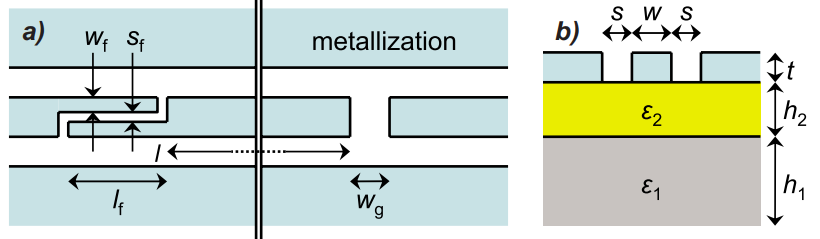
\includegraphics[height=0.3\textwidth,keepaspectratio]{CPWgoppl08}
\caption{\label{fig:CPWgoppl08} (a) CPW top view with finger capacitors (left) and gap capacitors (right). (b) CPW design cross section with a double layer substrate (yellow and grey)~\citep{doi:10.1063/1.3010859}.}
\end{figure}

The CPW cross-sectional view is shown in Fig.~\ref{fig:CPWgoppl08}(b) where the metal thickness is denoted by $t$ is most often referred to in the literature as $d$, therefore I will use the more conventional descriptor $d$. The central conductor width $W$ and the gap between the conductor and ground plane $S$ are values which impact $Q$ of the superconducting CPW waveguide. 
 
  

\subsection{CPW Q factor}
The quality factor describes how underdamped (high $Q$) or overdamped (low $Q$) a resonator is. The loaded quality factor is a parallel combination of internal and external (capacitive coupling) quality factors. The model for a LCR resonator quality factor utilised for derivation for the CPW by Yoshida in Ref.~\citep{402973}. The LCR resonator $Q$-factor:
\begin{equation}
\label{eq:LCRqfactor}
Q= \frac{\omega L}{R}
\end{equation}
is derived from considering that $Q$ is ratio of the total energy stored to the total energy lost per cycle\footnote{Useful link: http://www.techlib.com/reference/q.htm}. 

The lump inductance of the CPW is given as $L_{l} = L_{g}+L_{k}$ where the term for the kinetic inductance per unit length, $L_{k}$ only appears when the conductor is superconducting. The following inductance expressions where derived using conformal mapping in Ref~\citep{1347-4065-33-10R-5708} and Ref.~\citep{402973} based on a number of assumptions for a NbN film. (1) The wavelength of the transmitted wave is much greater than $W$. (2) The magnetic field outside the film acts as a perfect conductor. (3) $d < 2 \lambda_{L}$ where $\lambda_{L}=\sqrt{\frac{m_{e}}{\mu_{0} n_{e}q_{e}}}$  is the London (magnetic) penetration depth. The London penetration depth characterizes the distance to which a magnetic field penetrates into a superconductor until it becomes equal to $\exp(-1)$ times that of the magnetic field at the surface of the superconductor. (4) There is a uniform current density into the film. 

The results for the geometric inductance $L_{g}$ and $L_{k}$ are expressed as:
 \begin{equation}
\label{eq:geometricinductance}
L_{g} = \frac{\mu_{0}}{4}\frac{K(k')}{K(k)},
\end{equation}
\begin{equation}
\label{eq:kineticcapacitance}
L_{k} = \mu_{0}\frac{\lambda}{dW} g(S,W,d),
\end{equation} 
\noindent where $K(k)$ is the complete elliptic integral of the first kind with modulus $k = W /(W + 2S)$ and $k'=(1-k^{2})^{1/2}$. The geometrical factor $g(S , W, d)$ is:
\begin{equation}
\label{eq:geometricfactor}
g(S,W,d) = \frac{1}{2k'^{2}K(k)^{2}} \left [ \left ( -\ln{\frac{d}{4 W}}-\frac{W}{W+2S} \right ) \ln{\frac{d}{4(W+2S)}} + \frac{2(W+S)}{W+2S} \ln{\frac{S}{W+S}} \right ]
\end{equation}
\noindent accounting for the typographic error highlighted in Ref.~\citep{doi:10.1063/1.4773070}. $g(S,W,d)$ is not very sensitive to changes in $d$ and $S$ and $L_{k}$ increases as $d$ and $S$ decrease.  Additionally for $d < \lambda_{L}$, $L_{k}$ dominates $L_{l}$. 

Investigation of $L_{k}$ is completed by measuring the temperature of dependence of the resonant frequency given as:   
 \begin{equation}
\label{eq:tempresonantfrequency}
f_{c}=\frac{1}{2 l_{r} \sqrt{L(t)C_{g}}},
\end{equation}
\noindent where $t = T/T_{c}$. The geometric capacitance per until length $C_{g}$ is similarly derived using the conformal mapping method and is expressed as~\citep{doi:10.1063/1.3010859}: 
\begin{equation}
\label{eq:geometriccapacitance}
C_{g}=4\epsilon_{0}\epsilon_{eff}\frac{K(k_{0})}{K(ko')},
\end{equation}

\noindent and the lump inductance per unit length $L_{l}(t)$ is given as: 
\begin{equation}
\label{eq:templumpinductance}
L_{l}(t)=L_{g}+L_{k}(0) \theta_{k}(t),
\end{equation}
\noindent where the small temperature dependence of $L_{g}$ (for a thin electrode the magnetic field penetrates through) is neglected. The temperature dependence of $L_{g}$ is represented by $\theta_{k}(t)$ where the assumption is that  $\theta_{k} (t) \approx \theta_{\lambda_{L}} (t) ^{2}$ since from Eq.~\ref{eq:kineticcapacitance} it can be determined that $L_{k} \propto \sqrt{\lambda_{L}}$. Additionally, $\theta_{\lambda_{L}} (t)$ provides the temperature dependence of the London penetration depth such that $\lambda_{L}(t) = \lambda_{L}(0) \theta_{\lambda}(t)$. Good agreement to the experimental value calculated using Eq.~\ref{eq:kineticcapacitance} is achieved for the approximated expression:
\begin{equation}
\label{eq:tempLondonpentration}
\lambda_{L}(0) = 1.05 \times 10^{-3}\sqrt{\frac{\rho(T_{c})}{T_{c}}}m,
\end{equation} 

\noindent where $\rho(T_{c})$ is the normal state resistivity at $T=T_{c}$. For NbN films $T_{c} \approx$ 16 K~\citep{1347-4065-33-10R-5708} and for Nb $T_{c} \approx$ 8.8 K. 

\begin{figure}[H]
\centering
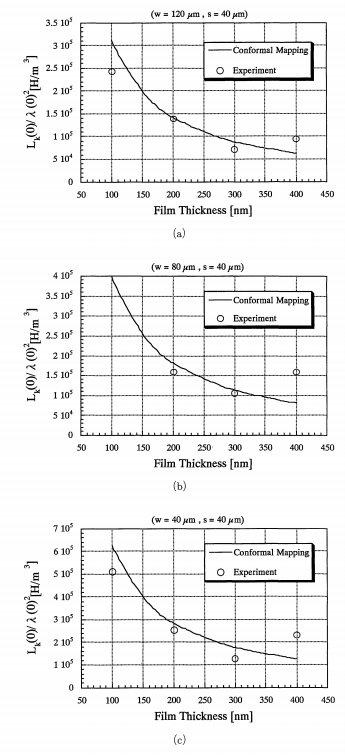
\includegraphics[height=1\textwidth,keepaspectratio]{LkvsT}
\caption{\label{fig:LkvsT} $d$ dependence of the $L_{k}$ of NbN CPW resonator for $S$= 40 $\mu$m where (a) $W$=120 $\mu$m, (b) $W$= 80 $\mu$m and (c) $W$=40 $\mu$m \citep{1347-4065-33-10R-5708}}
\end{figure}

The $\theta_{\lambda_{L}}$function of NbN is approximated using the local limit BCS theory since $\lambda_{L}/\xi>> 1 $, where $\xi$ is the coherence length. Superconducting CPW devices were fabricated on a Si substrate where $d$ ranges between 100-400 nm and $W$ ranges between 40-120 $\mu$m. The half wavelength resonator is built in and the CPW is coupled at both ends to connection lines such that the resonance frequency is measured as the temperature is swept. In the low temperature regime $f_{c}$ is constant and decreases rapidly as $T \rightarrow T_{c}$.  Fig.~\ref{fig:LkvsT} provides comparison of the theoretical and experimentally determined $L_{k}(0)$ which is expressed as $L_{k}(0)/\lambda_{L}(0)^{2}$ to provide independence of the sample $\lambda_{L}$. 





In Ref.~\citep{402973} an expression for the resistance per unit length is given as:

\begin{equation}
\label{eq:reistanceperunitlength}
R = \frac{\sigma_{1}}{\sigma_{2}} \omega L_{k},
\end{equation} 
where $\sigma= \sigma_{1}-i\sigma_{2}$ is the complex conductivity. The anomalous skin effect~\citep{10.1038/165239b0} describes the normal conductivity $\sigma_{N}$ of a metal at low temperatures, where extension of the conductivity description to superconductors was derived by Mattis and Bardeen~\citep{PhysRev.111.412}:  

  \begin{equation}
  \begin{aligned}
\label{eq:sigma1}
\frac{\sigma_{1}}{\sigma_{N}}=\frac{2}{\hbar \omega} \int_{\Delta}^{\infty} \left [ f(E)-f(E+\hbar \omega) \right ] \frac{(E^{2}+\Delta^{2}+\hbar \omega E)}{\sqrt{E^{2}-\Delta^{2}}\sqrt{(E+\hbar \omega)^{2})-\Delta^{2}}} dE \\
+\frac{1}{\hbar \omega} \int_{\Delta-\hbar \omega}^{-\Delta} \left [  1-2f(E+\hbar \omega)\right ] \frac{(E^{2}+\Delta^{2}+\hbar \omega E)}{\sqrt{E^{2}-\Delta^{2}}\sqrt{(E+\hbar \omega)^{2})-\Delta^{2}}} dE,
\end{aligned}
\end{equation} 
  \begin{equation}
\begin{aligned}
\label{eq:sigma2}
\frac{\sigma_{2}}{\sigma_{N}}= \frac{1}{\hbar \omega} \int_{\Delta-\hbar \omega, -\Delta}^{\Delta} \left [  1-2f(E+\hbar \omega) \right ] \frac{(E^{2}+\Delta^{2}+\hbar \omega E)}{\sqrt{\Delta^{2}-E^{2}} \sqrt{(E+\hbar \omega)^2-\Delta^{2}}},
\end{aligned}
\end{equation}   
\noindent where $\Delta = \frac{3.52}{2}k_{B}T_{c}$ is half of the superconducting energy gap for Nb from BCS theory. The temperature dependence of $\Delta$ is given as $\Delta (T) = \Delta(0) \sqrt{1-\frac{T}{T_{c}}}$. The second term of Eq.~\ref{eq:sigma1} does not appear unless $\hbar \omega > 2 \Delta$ where for this case the lower limit of the integral in Eq.~\ref{eq:sigma2} is $- \Delta$ (instead of $\Delta - \hbar \omega$). 
In Fig.~\ref{fig:conductivitybeck} the theoretical investigation of the temperature dependence of $\sigma_{1}/\sigma_{N}$ and $\sigma_{2} / \sigma_{N}$ completed in Ref.~\citep{mattbeck} is shown. 

\begin{figure}[H]
\centering
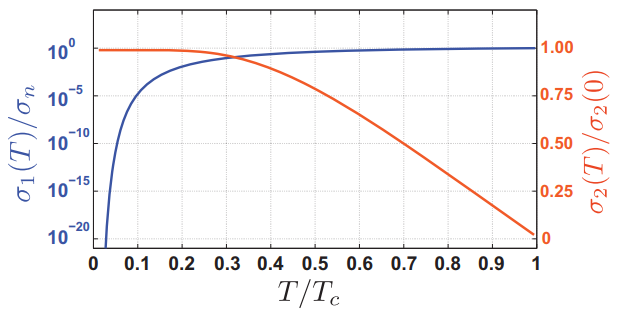
\includegraphics[height=0.4\textwidth,keepaspectratio]{conductivitybeck}
\caption{\label{fig:conductivitybeck} The normalised Mattis-Bardeen conductivities verse reduced temperature where $\sigma_{1} / \sigma_{N}$ is shown by the blue curve and $\sigma_{2} / \sigma_{N}$ is shown by the red curve for $f_{c}$ = 5 GHz \citep{1347-4065-33-10R-5708}}
\end{figure}


Finally in Ref.~\citep{doi:10.1063/1.4962172} the expression for the quasi-particle limited $Q$ for a superconducting CPW resonator is given as:
\begin{equation}
\label{eq:Qquasilimited}
Q_{qp} = \frac{\sigma_{2}}{\sigma_{1}} \left ( 1 + \frac{L_{g}}{L_{k}} \right ).
\end{equation} 
where design and characterisation of a superconducting CPW device is fabricated to enable strong coupling to a single trapped Rydberg atom. This is achieved through in addition of copper electrodes at a voltage antinode of the resonator enchancing the zero-point electric fields of the resonator at the point in space the atom is trapped (40 $\mu$m above the CPW surface). This scheme can achieve the strong coupling limit. (In Ref.~\citep{PhysRevA.89.010301} the approach of coupling the electric dipole moment to the zero point electric field is discussed.) Note that the complex surface impedance of the superconductor is $R$+i$L_{k}$. Fig.~\ref{fig:qfactorbeck}(a) illustrates the behaviour of the normalised current density of a CPW device. Fig.~\ref{fig:qfactorbeck}(b) shows the series of quarter wavelength CPW resonators used to probe the dependence of the resonator $Q$ on geometry where capacitive coupling to the transmission line is achieved. Comparison of the theoretical and experimentally computed internal $Q$ factor is shown, for a Nb film of $d$= 95 nm and $\Delta (0) =10^{-3}$ eV, in Fig~\ref{fig:qfactorbeck}(c).  

\begin{figure}[H]
\centering
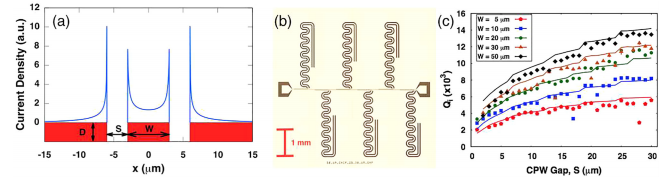
\includegraphics[height=0.27\textwidth,keepaspectratio]{qfactorbeck}
\caption{\label{fig:qfactorbeck} (a) The supercurrent density (blue line) for a CPW where $W$ = 6 $\mu$m and $S$ = 3 $\mu$m and $\lambda_{L}(0) = 87$ nm. (b) Optical micrography of the multiplexed CPW resonator chip. (c) Internal CPW $Q$ as a function of $W$ and $S$ at $T=T_{c}$. The theoretical line breaks are due to using slightly different $f_{c}$ values \citep{ doi:10.1063/1.4962172}.}
\end{figure}


\subsubsection{Results}
The results of plotting $\sigma_{2}/ \sigma_{N}$ following expected results as the imaginary component of $\sigma$ decrease to zero at $T_{c}$. However, the behaviour of $\sigma_{1} / \sigma_{N}$ vs. $T/T_{c}$ shown in Fig.~\ref{fig:sigma1sigma2} deviates from Fig.~\ref{fig:conductivitybeck}
    
    \begin{figure}[H]
    \centering
    \begin{subfigure}[b]{0.45\textwidth}
        \centering
        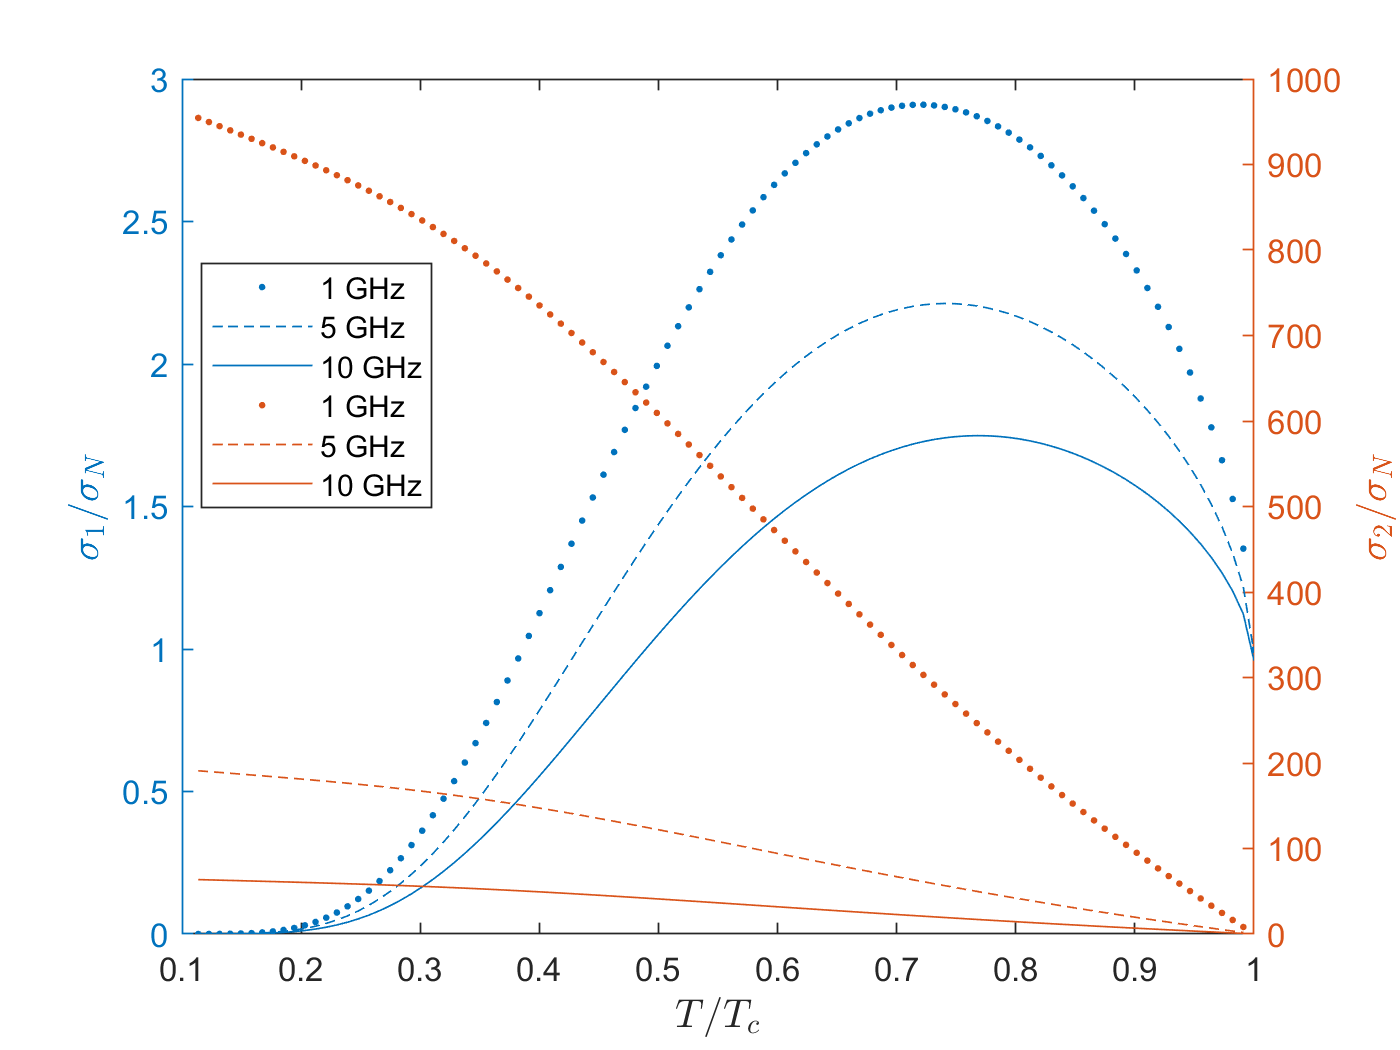
\includegraphics[width=\textwidth]{sigma1sigma2}
        \caption{\label{fig:sigma1sigma2}}
    \end{subfigure}
%     \hfill
         \begin{subfigure}[b]{0.45\textwidth}
        \centering
        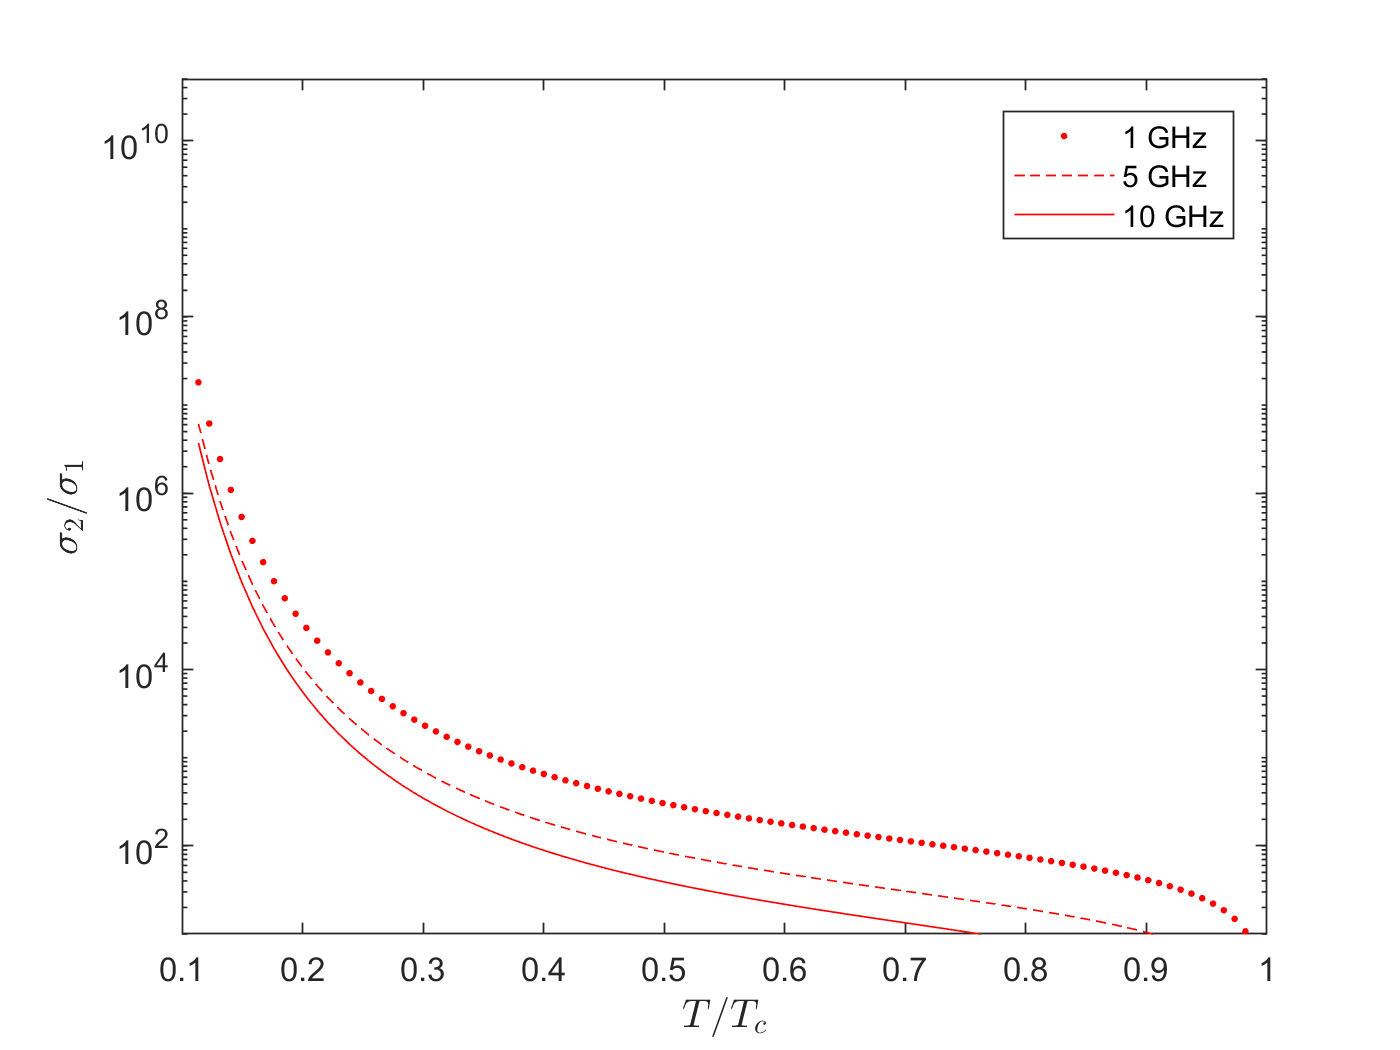
\includegraphics[width=\textwidth]{ratiosigma2tosigma1}
   \caption{\label{fig:ratiosigma2tosigma1}}
   \end{subfigure}
   \caption{(a) $\sigma_{1} / \sigma_{N}$ (blue), $\sigma_{2} / \sigma_{N}$ (red) and (b) $\sigma_{2} / \sigma_{1}$ vs. $t=T/T_{c}$ for a selection of input frequency values. $T_{c} = 8.8$ K.}
   \label{fig:mairflaigthesisreplicate}
    \end{figure}

The next step is to verify the results of Yoshida for a NbN film in Ref.~\citep{402973} at $T$ = 4.2 K. Approximate data points for Ref.~\citep{402973} are given by the black circles.   



\noindent \textit{Remember to make a note on the Clem paper and why it is not applicable to the thick film case.}

\noindent \textit{Points I am still uncertain of:}



\noindent \textit{- The internal and external CPW components and Q factor}